\section{Empirical Evaluation}
  
In this section we compare the solutions for traffic networks modeled as a QTM
before and after the introduction of a light rail.
%
We consider both fixed-time control, i.e., a non-adaptive control plan, and
optimized adaptive control obtained by solving the
MILP~(\ref{eq:objFunc},~\ref{c:turnProb}--\ref{c:pd:holdTransit}).
%
The obtained solutions are simulated using a microsimulator and their total
travel time and observed delay distribution are used as comparison metrics.
%
Our hypothesis is that the optimized adaptive approach is able to mitigate the
impact of introducing light rail w.r.t.\ both metrics.
%
In the remainder of this section, we present the traffic networks considered in
the experiments, our methodology, and the results.






\subsection{Networks}

\begin{figure}[t!]
\centering
%  trim={<left> <lower> <right> <upper>}
\begin{subfigure}{0.47\textwidth}
\label{fig:net:arterial}
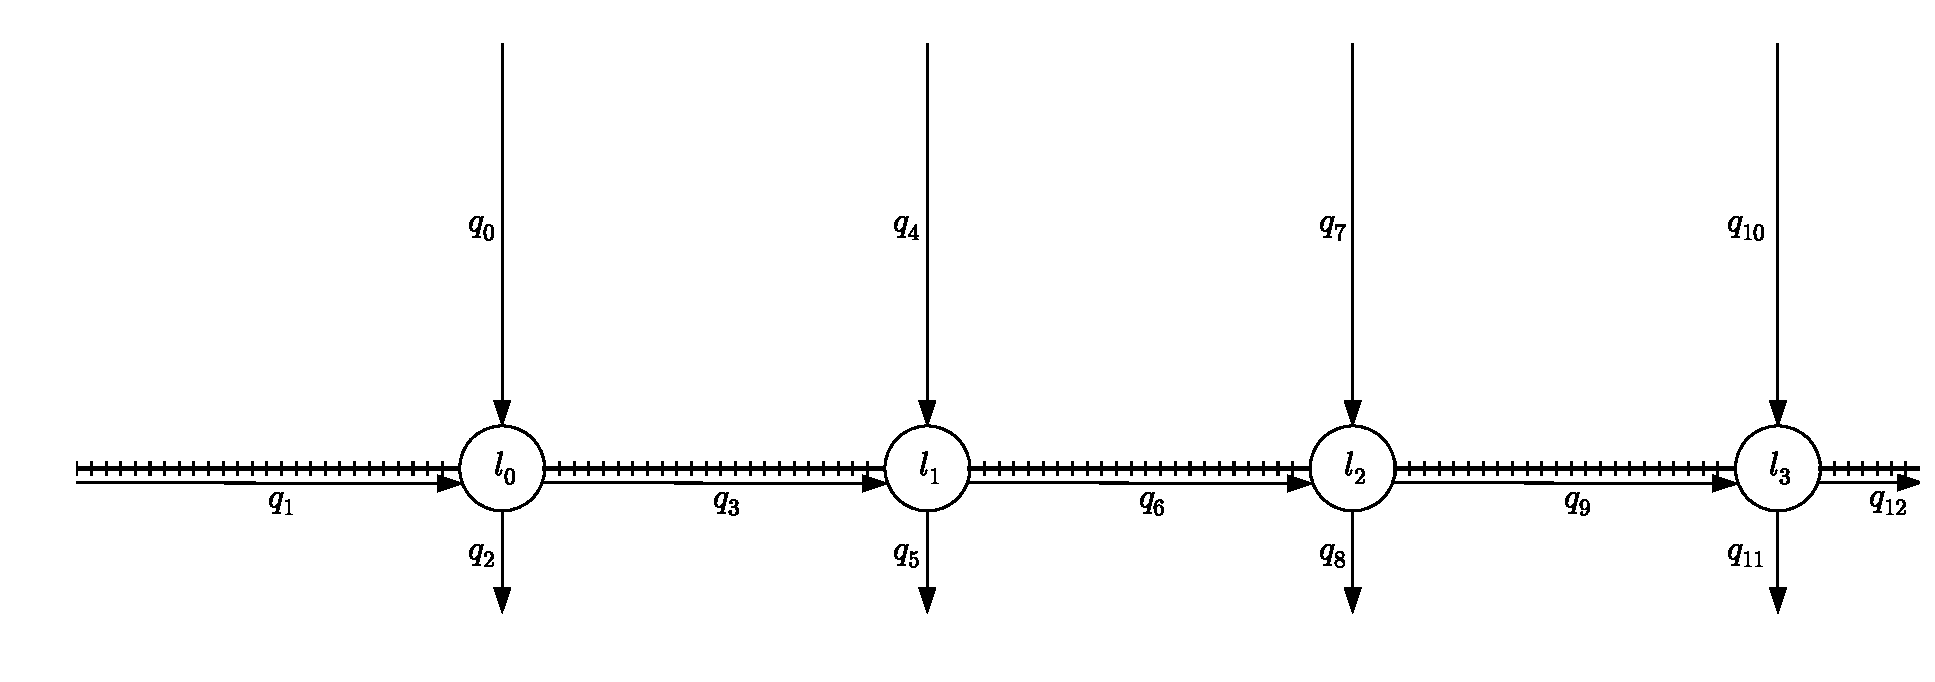
\includegraphics[trim={0 20 0 20},width=\linewidth]{network1.pdf}
\caption{~}
\vspace{3mm}
\end{subfigure}
\begin{subfigure}{0.50\textwidth}
\label{fig:net:grid}
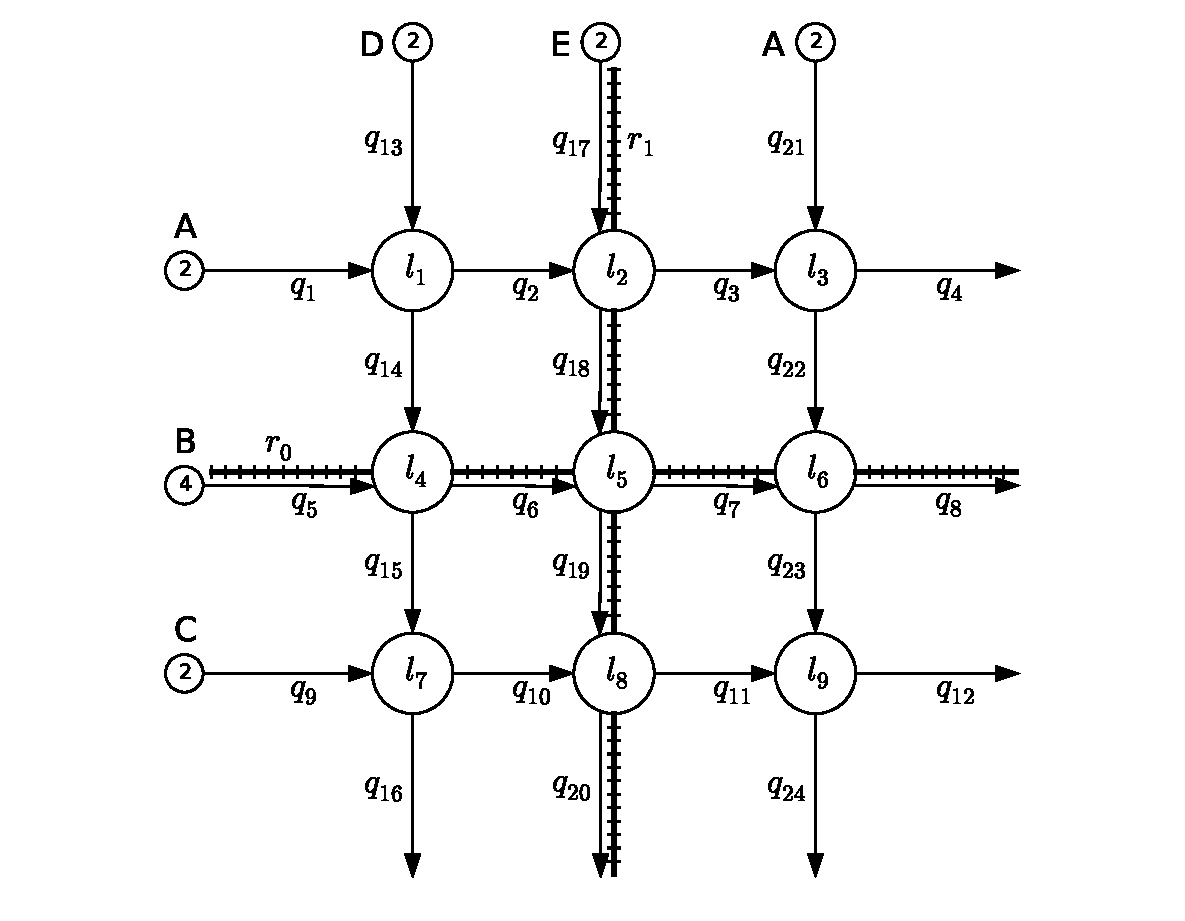
\includegraphics[trim={0 20 0 20},width=\linewidth]{network2.pdf}
\caption{~}
\end{subfigure}
\caption{Networks used to evaluate the performance:
  (a) an arterial road with parallel light rail;
  (b) an urban grid with crisscrossing streets and light rail.
%
%(d) Demand profile of the queues marked as \qLowTraf,
  %\qHighTraf, and \qVarTraf for our experiments.
}
\label{fig:networks}
\end{figure}


We consider two networks of differing complexity: an arterial crossed by four
side streets (\cref{fig:net:arterial}) and a 3-by-3 grid (\cref{fig:net:grid}).
%
The queues receiving cars from outside of the network are
marked in \cref{fig:networks} and we refer to them as input queues.
%
The maximum queue capacity~(\QMAX{i}) is 60 vehicles for non-input queues and
infinity for input queues to prevent interruption of the input demand due to
spill back from the stop line. 
%
The free flow speed is 50 km/h and the traversal time of each queue $i$~(\QDELAY{i}) is set at 30s,
except for the output queues on Network 1 where the traversal
time is 10s.
%
For each street, flows are defined from the head of each queue $i$ into the tail
of the next queue $j$;
%
there is no turning traffic ($\FTURN{i}{j}=1$), and the maximum flow rate
between queues, \FMAX{i}{j}, is set at 0.5 vehicles/s.
%
All traffic lights have two phases, north-south and east-west, and for each
traffic light \tl and phase $k$, \PTMIN{\tl}{k} is 10s, \PTMAX{\tl}{k} is 30s,
\CTMIN{\tl} is 20s, and \CTMAX{\tl} is 60s.



%\subsection{Fixed-Time Control Constraints}
%
%We simulate a fixed-time traffic light controller by employing the QTM to
%optimize a fixed phase duration, \PTFIXED{\ell}{k}, over the
%planning horizon.
%%
%We implement this by replacing the bounds constraints on $\pd[n]{\ell}{k}$
%($\pd[n]{\ell}{k} \le \PTMAX{\ell}{k}$ and \ref{c:minPhase}), with fixed duration
%constraints, employing the \textit{big-M} method to apply the constraints only
%while the phase is inactive, where 
%$\PTFIXED{\ell}{k} \in [\PTMIN{\ell}{k}, \PTMAX{\ell}{k}]$.
%%
%\begin{cAlign}
%        \pd{\ell}{k} &\le \PTFIXED{\ell}{k} + \PTMAX{\ell}{k} \p[n]{\ell}{k}
%  \tagconstrain{c:pd:fixedUB}\\
%%
%  \pd{\ell}{k} &\ge \PTFIXED{\ell}{k} - \PTMAX{\ell}{k} \p[n]{\ell}{k}
%  \tagconstrain{c:pd:fixedLB}
%\end{cAlign}
% 
%Constraints \ref{c:pd:fixedLB} and \ref{c:pd:fixedUB} are only applied for time
%intervals $n$ where $\tn[n] > \CTMAX{\tl}$, to allow the controller to select an
%optimized phase offset at the start of each plan.
%%TODO talk about how the fixed phase times fit around transit crossings.
%


\subsection{Experimental Methodology}


\begin{figure}[t!]
\centering
%  trim={<left> <lower> <right> <upper>}
%trim={0 10 0 2}
\scriptsize{Slow light rail}\\
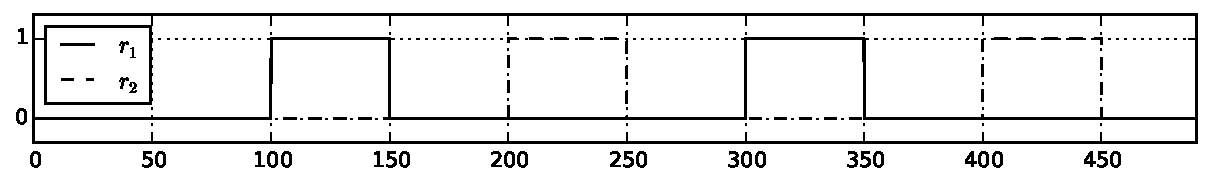
\includegraphics[width=0.45\textwidth]{Transit1_sched.pdf}
\scriptsize{Fast light rail}\\
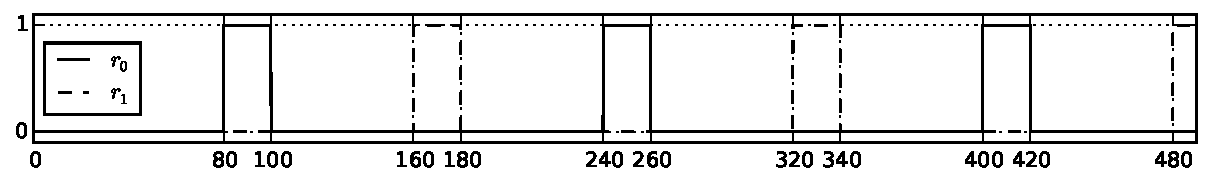
\includegraphics[width=0.45\textwidth]{Transit2_sched.pdf}
\caption{Light rail schedule functions.}
\label{fig:transits}
\end{figure}



We evaluate each network using both fixed-time control and the optimized
adaptive control in two scenarios: before the introduction of light rail and
after.
%
For the latter scenario, we consider the two different light rail schedules
depicted in \cref{fig:transits}:
%
a slow light rail with a crossing duration of 50s, a period of 200s, and a
travel time of 100s between lights;
%
and a fast light rail with a crossing duration of 20s, period of 160s, and
travel time of 80s between lights.
%
On Network 2, the North-South schedule is offset by 100s for the slow light rail
and 80s for the fast light rail to avoid a collision at $l_5$.



\begin{figure}[t]
\centering
%  trim={<left> <lower> <right> <upper>}
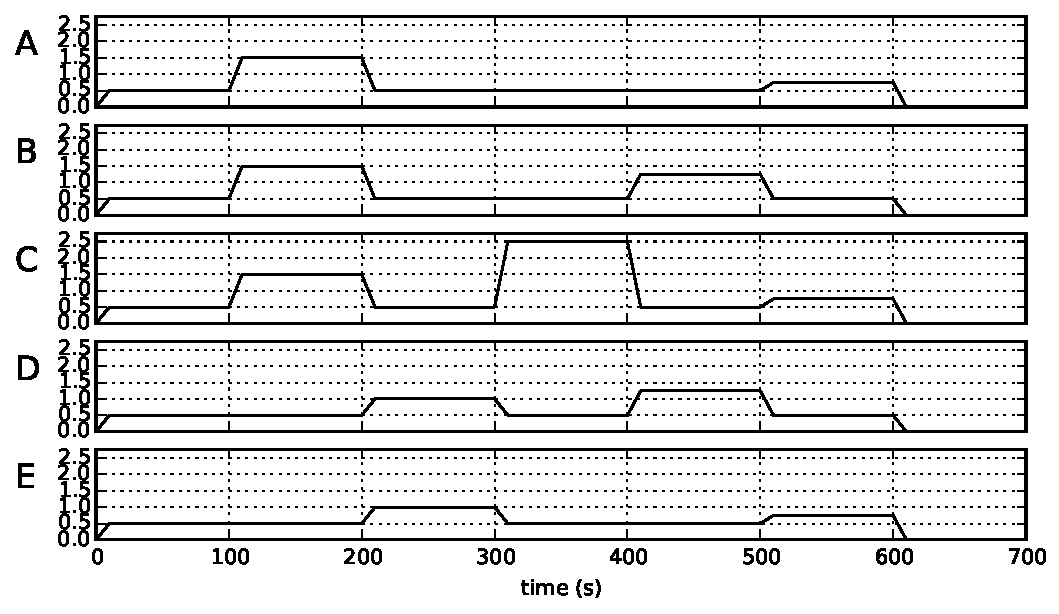
\includegraphics[width=0.47\textwidth]{demand_profiles.pdf}
\caption{Weight functions for generating demand profiles.}
\label{fig:demand_profiles}
\end{figure}


%
%% TODO(fwt): improve this description and say upfront that the demand levels
%% are parametrized by \alpha
%
Each network is evaluated at increasing demand levels up to the point where
$\inq{i}$ becomes saturated.
%
%% TODO(fwt): we need to clarify that both approaches have access to the whole
%% "future", i.e., perfect information about the incoming cars.
%
For each demand level, traffic is injected into the network in bursts for 600s,
and the number of cars entering the network through $i$ at time $n$ is defined
as $\QIN{i}{n} = \mathrm{max}(\alpha \beta \mathrm{w}_i(\tn[n]),\beta)$ where:
%
$\mathrm{w}_i$ is the weight function in \cref{fig:demand_profiles}
corresponding to the letter label of $i$ in \cref{fig:networks};
%
$\beta$ is the maximum inflow rate in vehicles per \DT, as annotated at the
start of queue $i$ in \cref{fig:networks}; and
%
$\alpha \in (0,2]$ is the scaling factor for the demand level being evaluated.


For each evaluation, we first generate a signal plan using QTM configured as
either an optimized adaptive controller or a fixed-time controller.
%
We use a problem horizon \TMAX large enough, typically in the range 1000s --
1500s, to allow all traffic to clear the network, what let us measure the
incurred delay in all the cars.
%
Next, we microsimulate the signal plans on their respective the networks using
the Intelligent Driver Model (IDM)~\cite{treiber2000congested}.
%
For the microsimulation, all vehicles have identical IDM parameters: length
$l=3$~m, desired velocity $v_0 = 50$~km/h, safe time headway $T=1.5$~s, maximum
acceleration $a=2 \text{ m/s}^2$, desired deceleration $b = 3 \text{ m/s}^2$,
acceleration exponent $\delta = 4$, and jam distance $s_0 = 2$~m.
%
We follow the same demand profiles used for computing the signal plans for the
microsimulation.


For all experiments, we used Gurobi as the MILP solver running on a
heterogeneous cluster with 2.8GHz AMD Opteron~4184, 3.1GHz AMD Opteron~4334 (12
cores each), and 2Ghz Intel Xeon E5405 (4 cores). We use 4 cores for each run of
the solver.
%
We limit the MIP gap accuracy to 0.02\% and 0.1\% for the arterial and grid
networks, respectively.
%
Due to Gurobi's stochastic strategies, runtimes for the solver can vary, and we
do not set a time limit.
%
The optimized adaptive solution are typically found in real time (less than
200s), while fixed-time plans can take significantly longer (on average 4000s
for a 1000s horizon); however, once the fixed-time solution is found, it can be
deployed indefinitely.
%
%\toIain{Do you have the cputimes by any chance in your log files so that we
%could say what is the average?}




\subsection{Results}


\begin{figure*}[t]
%
\centering
%  trim={<left> <lower> <right> <upper>}
\begin{subfigure}{0.49\textwidth}\label{fig:arterial:delayCurve}
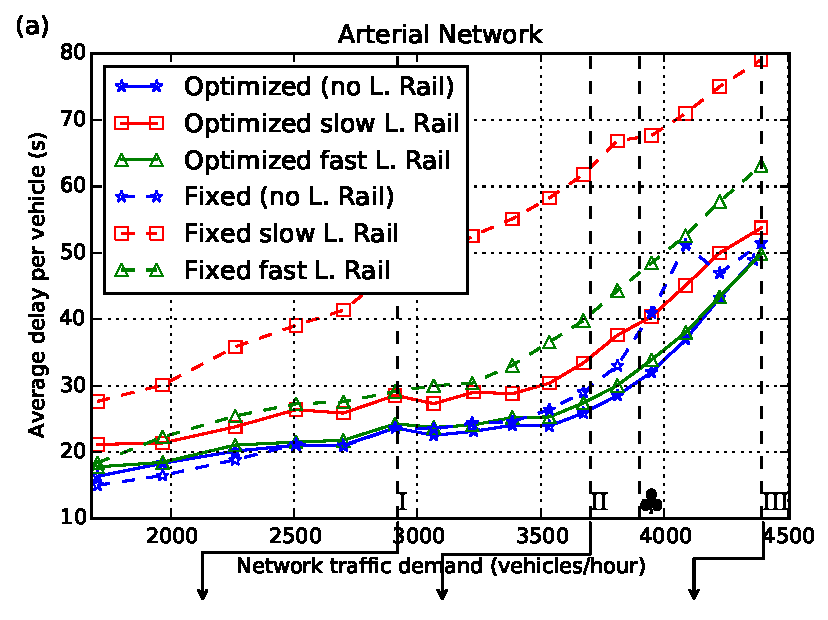
\includegraphics[keepaspectratio,width=\linewidth]{network1_delay.pdf}
\caption{~}
\end{subfigure}
\begin{subfigure}{0.49\textwidth}\label{fig:grid:delayCurve}
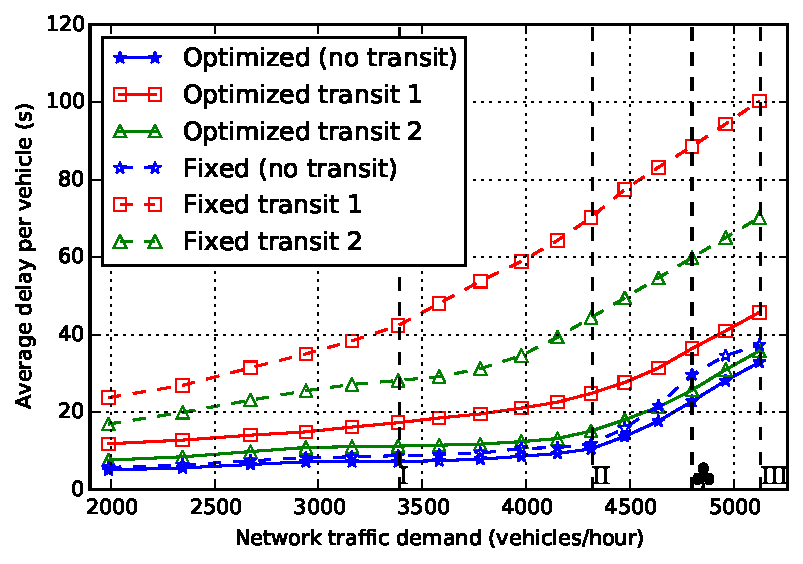
\includegraphics[keepaspectratio,width=\linewidth]{network2_delay.pdf}
\caption{~}
\end{subfigure}
\begin{subfigure}{0.49\textwidth}\label{fig:arterial:boxplot}
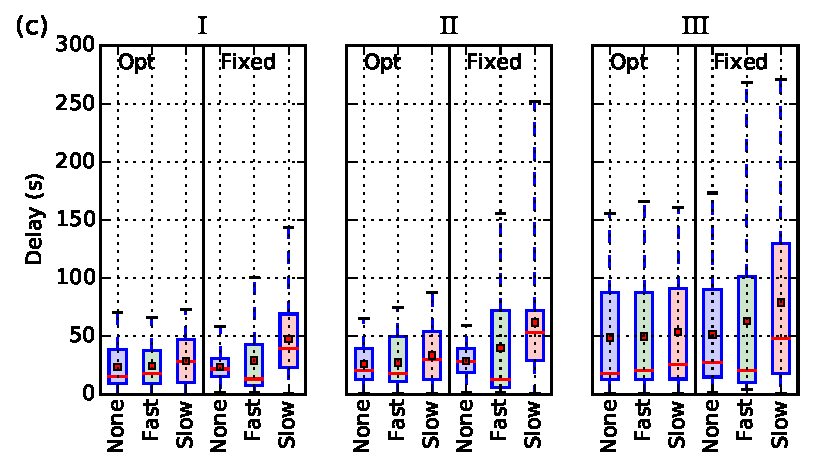
\includegraphics[keepaspectratio,width=\linewidth]{network1_boxplots.pdf}
\caption{~}
\end{subfigure}
\begin{subfigure}{0.49\textwidth}\label{fig:grid:boxplot}
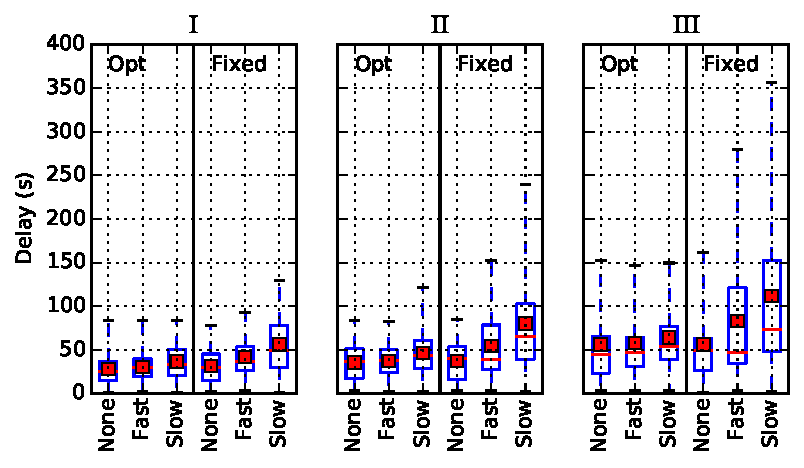
\includegraphics[keepaspectratio,width=\linewidth]{network2_boxplots.pdf}
\caption{~}
\end{subfigure}
%
\caption{Average delay by the network demand for the arterial (a) and grid (b)
networks. Box plots representing the observed distribution of delay for 3
different values of demand for each network (c,d). The mean is presented as a
red square in the box plots.}
%
\label{fig:delayCurveAndBoxplot}
%
\end{figure*}


\cref{fig:arterial:delayCurve,fig:grid:delayCurve} show, for each network, the
average delay per vehicle as a function of demand for both optimized fixed-time and
optimized adaptive control approaches in three scenarios: before the light rail and after
the installation of light rail using the slow and the fast schedules.
%
As we hypothesized, optimized adaptive control is able to mitigate the impact of
the introduction of light rail and it marginally increases the average delay
when compared with the average delay produced by fixed-time controller
\textbf{before} the light rail.
%
Moreover, as shown in \cref{fig:arterial:boxplot,fig:grid:boxplot}, the
optimized adaptive controller also produces better signal plans than the
fixed-time controller, i.e., plans with smaller median, third quartile, and
maximum delay.
%
Overall our experiments, the maximum observed delay for the optimized adaptive
signal plans after the introduction of light rail is no more than
%
%% TODO(fwt): The results improved and we can (and have to) provide a tighter
%% bound.
%
the double of the maximum delay before the light rail.
%
\cref{fig:network_hist} provides more details on the behavior of the signal
plans for demand level $\rm II$~(\cref{fig:demand_profiles}) by showing the
cumulative number of cars by number of observed stops.
%
Note that in \cref{fig:network1_slow:hist:arterial,fig:network1_slow:hist:side}
the fixed-time controller chooses to prioritize the arterial over the side
streets, but overall (\cref{fig:network1_slow:hist}) the optimized controller
does better with less stops at all frequencies.


\begin{figure*}[t!] \centering
%  trim={<left> <lower> <right> <upper>}
\begin{subfigure}{0.49\textwidth}\label{fig:arterial:impact:t1}
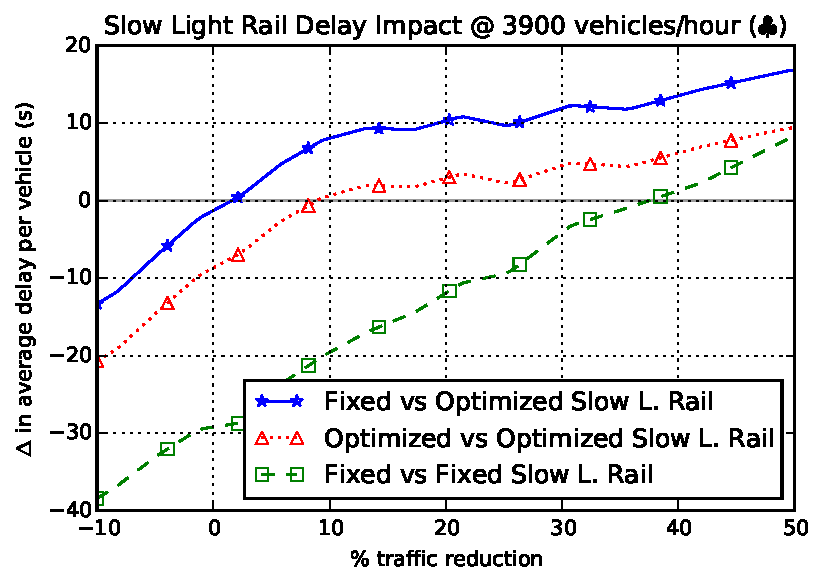
\includegraphics[keepaspectratio,width=\linewidth]{network1_t1_reduction.pdf}
\caption{~}
\end{subfigure}
\begin{subfigure}{0.49\textwidth}\label{fig:grid:impact:t1}
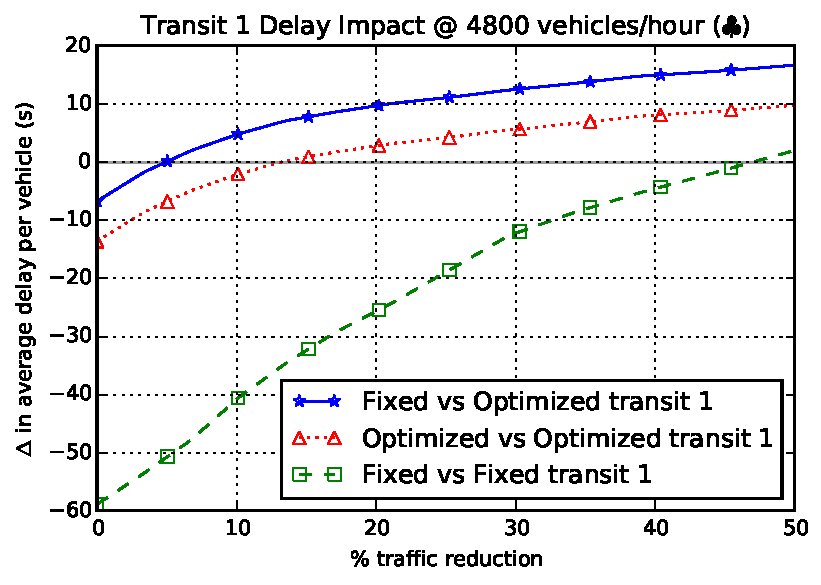
\includegraphics[keepaspectratio,width=\linewidth]{network2_t1_reduction.pdf}
\caption{~}
\end{subfigure}
\begin{subfigure}{0.49\textwidth}\label{fig:arterial:impact:t2}
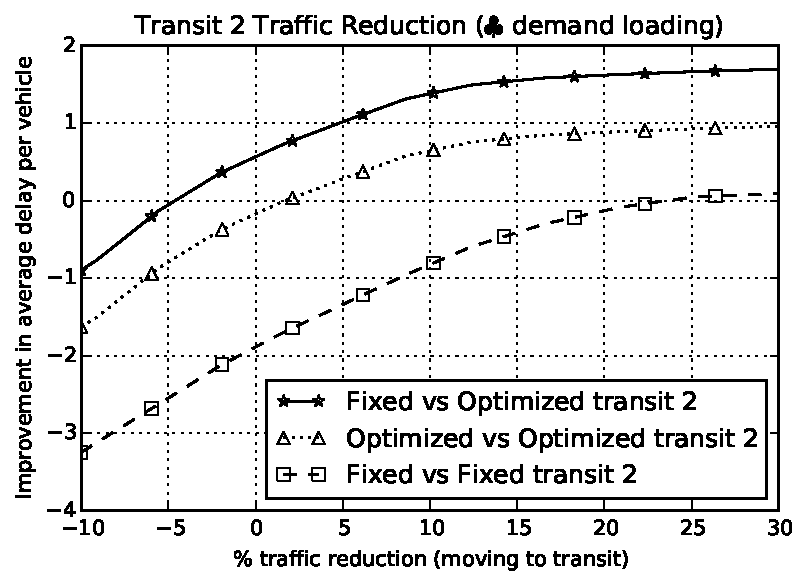
\includegraphics[keepaspectratio,width=\linewidth]{network1_t2_reduction.pdf}
\caption{~}
\end{subfigure}
\begin{subfigure}{0.49\textwidth}\label{fig:grid:impact:t2}
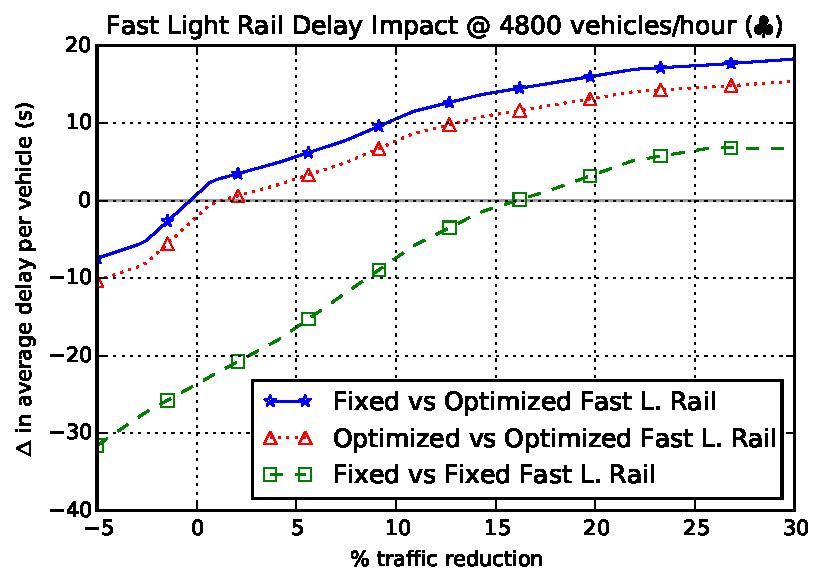
\includegraphics[keepaspectratio,width=\linewidth]{network2_t2_reduction.pdf}
\caption{~}
\end{subfigure}
%
\vspace{-2mm}
\caption{Impact on average delay for the arterial (first column) and grid
(second column) networks for both light rail schedules (rows) in different
scenarios (curves) of traffic control system before and after installation of
light rail.
%%
The x-axis is the percentage of cars switching to the public transportation
and the y-axis is the impact after the light rail is installed.
%
Negative impact represents increase in average delay.
%
The vehicle demand for (a-d) are marked as $\clubsuit$ in their
respective plots in \cref{fig:delayCurveAndBoxplot}.}
%
\label{fig:impact} \end{figure*}



To further illustrate the benefits of using optimized adaptive control to
minimize the impact of adding light rail to traffic network, \cref{fig:impact}
shows the impact on average delay as a function of the percentage of cars that
are switching to the light rail.
%
In these plots, the demand level is fixed
%
%and its value is labeled by $\clubsuit$ in \cref{fig:delayCurveAndBoxplot},
%
and higher values are better~(i.e., there is a decrease in the average delay)
and zero means that there is no change after installing light rail.
%
For the three combinations of before and after policies presented,
%
%(we omit the case of using optimized adaptive before the light rail and
%fixed-time after the light rail),
%
we can see that, while keeping the fixed-time controller requires from 7.5\% to
40\% of the drives to switch to light rail in order to obtain the same average
delay as before its installation, the optimized adaptive approach requires only
from 2.5\% to 10\% of the drivers to switch when already using optimized
adaptive control \textbf{before} the light rail.
%
When compared fixed-time before the light rail and optimized adaptive after, the
average delay stays the same if only the 2\% and 5\% of the drives switch to the
light rail when considering the slow light rail schedule in the arterial and
grid networks, respectively;
%
moreover, the average delay \textbf{decreases} for both networks using the fast
light rail schedule even if no driver switches to the newly installed public
transportation.

\begin{figure*}[t!] \centering
%  trim={<left> <lower> <right> <upper>}
%
\begin{subfigure}{0.68\textwidth}
  \centering
  \footnotesize{Network 1}
\end{subfigure}
\begin{subfigure}{0.2\textwidth}
  \centering
  \footnotesize{Network 2}
\end{subfigure}\\[2mm]
\begin{subfigure}{0.275\textwidth}\label{fig:network1_slow:hist:arterial}
  \centering
  \qquad \qquad \footnotesize{Arterial}
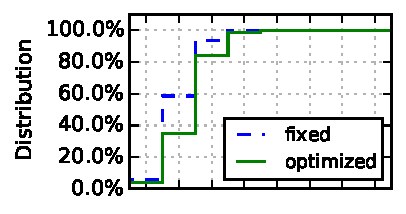
\includegraphics[keepaspectratio,width=\linewidth]{network1_hist_slow_arterial.pdf}
\end{subfigure}
%
\begin{subfigure}{0.2\textwidth}\label{fig:network1_slow:hist:side}
  \centering
  \footnotesize{Side Streets}
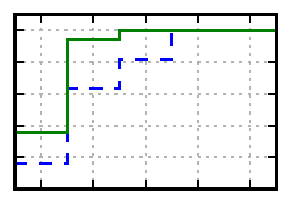
\includegraphics[keepaspectratio,width=\linewidth]{network1_hist_slow_side.pdf}
\end{subfigure}
%
\begin{subfigure}{0.2\textwidth}\label{fig:network1_slow:hist}
  \centering
  \footnotesize{Overall}
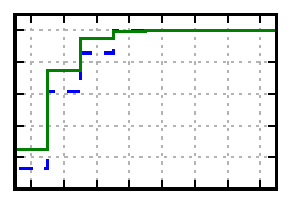
\includegraphics[keepaspectratio,width=\linewidth]{network1_hist_slow.pdf}
\end{subfigure}
%
\begin{subfigure}{0.2\textwidth}\label{fig:network2_slow:hist}
  \centering
  \footnotesize{Overall}
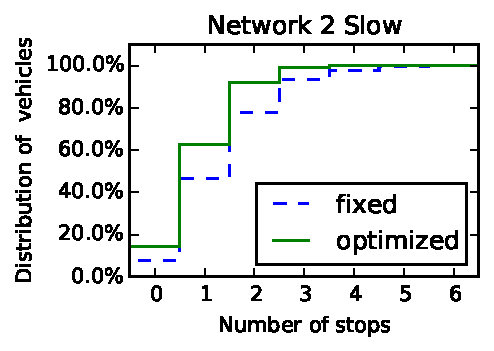
\includegraphics[keepaspectratio,width=\linewidth]{network2_hist_slow.pdf}
\end{subfigure}
%
\begin{subfigure}{0.28\textwidth}\label{fig:nwrwork1_fast:hist:arterial}
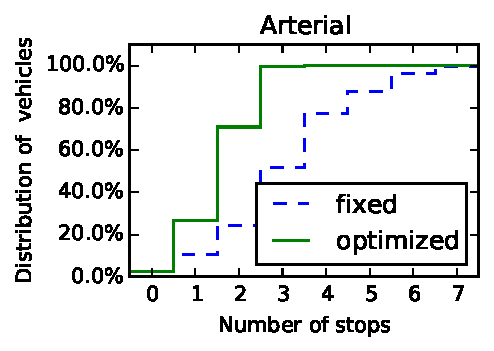
\includegraphics[keepaspectratio,width=\linewidth]{network1_hist_fast_arterial.pdf}
\end{subfigure}
\begin{subfigure}{0.2\textwidth}\label{fig:network1_fast:hist:side}
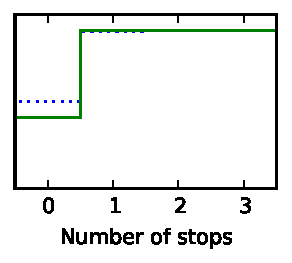
\includegraphics[keepaspectratio,width=\linewidth]{network1_hist_fast_side.pdf}
\end{subfigure}
\begin{subfigure}{0.2\textwidth}\label{fig:network1_fast:hist}
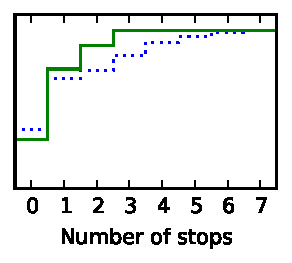
\includegraphics[keepaspectratio,width=\linewidth]{network1_hist_fast.pdf}
\end{subfigure}
\begin{subfigure}{0.2\textwidth}\label{fig:network2_fast:hist}
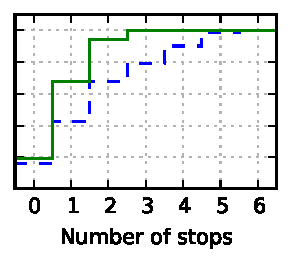
\includegraphics[keepaspectratio,width=\linewidth]{network2_hist_fast.pdf}
\end{subfigure}
\vspace{-2mm}
\caption{Impact of fast light rail on number of stops for Network 1. Top row is for the slow light rail schedule. Bottom row is for the fast light rail schedule}
\label{fig:network_hist}
\end{figure*}

\cref{fig:network1_microsim} shows microsimulation time-distance plots for several streets in Network 1. The y-axis of the plot
shows the distance along the street, and the x-axis shows the evolution over time. Each colored trace represents the journey of a vehicle along the street. Traffic signals at fixed distances down the street appear as black horizontal dashed lines, where a solid bar represents that the phase is inactive, that the light is red, and traffic cannot pass. Where the line is broken the phase is active, the light is green and cars can proceed past. The time-distance plots capture the queueing behaviour of the traffic as each vehicle decelerates when approaching congested traffic, or red or amber light ahead. When the trace of a vehicle is horizontal, it has become stationary.
From the microsimulation time-distance plots of the side streets (\cref{fig:network1_microsim}) we can see that the fixed-adaptive controller has prioritized the arterial phase duration over the side street duration, to achieve coordinated ``green corridors'', sized for the average traffic density in the network, and suffers from accumulative queue build up in the side streets following each transit of the light rail.
Conversely, the optimized controller is able to clear out the queue build up in the side streets by increasing the phase time of the side street for a cycle after the transit has passed through, and then returns to a schedule that prioritises the arterial depending on the changes in traffic density. When the traffic density in the arterial is higher than the side streets then the optmized controller will coordinate ``green corridors'' along the arterial.\footnote{The supplementary material further elucidates this point.}

\begin{figure*}[t!] \centering
%  trim={<left> <lower> <right> <upper>}
\begin{subfigure}{0.49\textwidth}
  \centering
  \footnotesize{Fixed Controller Side Street $q_5$ to $q_6$}
\end{subfigure}
\begin{subfigure}{0.49\textwidth}
  \centering
  \footnotesize{Optimized Controller Side Street $q_5$ to $q_6$}
\end{subfigure}
\begin{subfigure}{0.49\textwidth}\label{fig:network1_microsim:fixed_side:slow_lr}
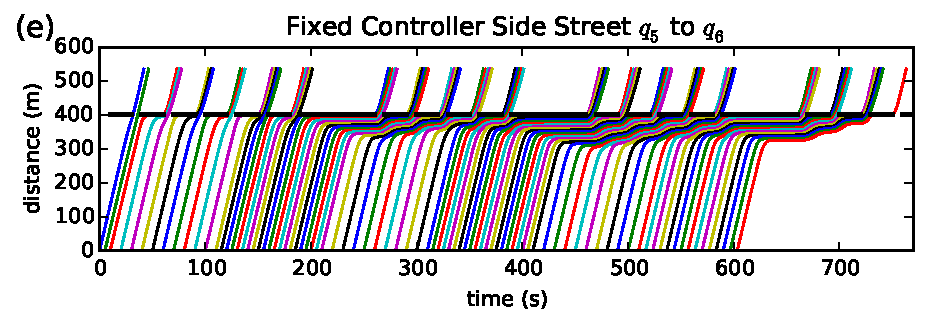
\includegraphics[keepaspectratio,width=\linewidth]{network1_microsim_fixed_slow_side.pdf}
\caption{}
\end{subfigure}
\begin{subfigure}{0.49\textwidth}\label{fig:network1_microsim:opt_side:slow_lr}
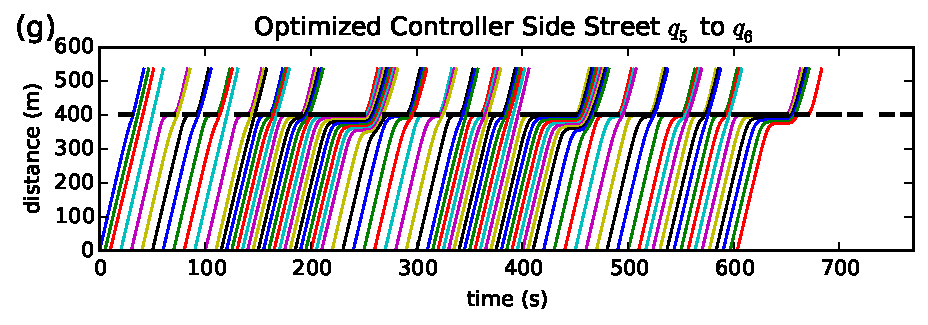
\includegraphics[keepaspectratio,width=\linewidth]{network1_microsim_opt_slow_side.pdf}
\caption{}
\end{subfigure}
\begin{subfigure}{0.49\textwidth}
  \centering
  \footnotesize{Fixed Controller Arterial $q_2$ to $q_{10}$}
\end{subfigure}
\begin{subfigure}{0.49\textwidth}
  \centering
  \footnotesize{Optimized Controller Arterial $q_2$ to $q_{10}$}
\end{subfigure}
\begin{subfigure}{0.49\textwidth}\label{fig:network1_microsim:fixed_side:fast_lr}
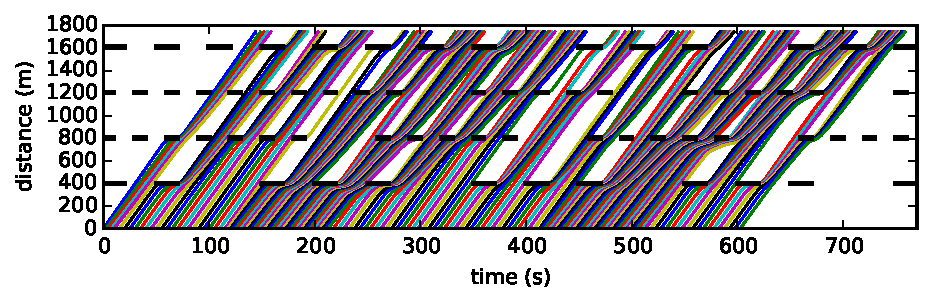
\includegraphics[keepaspectratio,width=\linewidth]{network1_microsim_fixed_slow_arterial.pdf}
\caption{}
\end{subfigure}
\begin{subfigure}{0.49\textwidth}\label{fig:network1_microsim:opt_side:fast_lr}
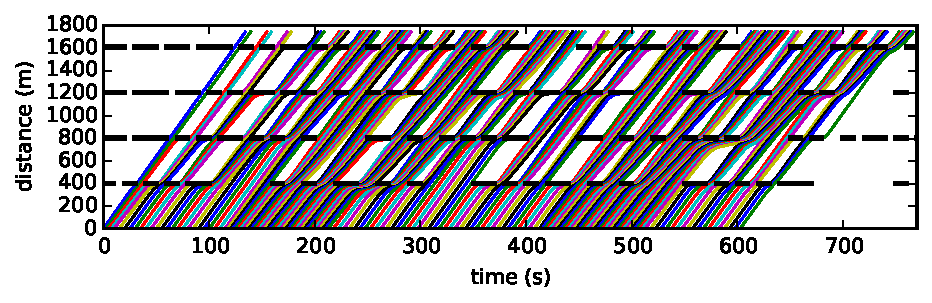
\includegraphics[keepaspectratio,width=\linewidth]{network1_microsim_opt_slow_arterial.pdf}
\caption{}
\end{subfigure}
%
%\vspace{-5mm}
\caption{Microsimulation time-distance plots of side street $q_5$ to $q_6$ and arterial $q_2$ to $q_{13}$ in Network 1 with the slow light rail schedule. The fixed-adaptive controller has prioritized the arterial phase duration (c) over the side street duration (a) and suffers from accumulative queue build up in the side streets following each transit of the light rail.
%
The optimized controller is able to clear out the queue build up in the side streets by increasing the phase time of the side street (b) for a cycle after the transit has passed through, and then returns to a schedule that prioritizes the arterial (d) depending on the changes in traffic density.}
%
\label{fig:network1_microsim}
\end{figure*}

